%\documentclass[article,pdftex,10pt,a4paper,twocolumn]{article}
\documentclass[article,pdftex,12pt,a4paper]{article}
\usepackage[authoryear]{natbib}
\usepackage{graphics}

\usepackage{url}\urlstyle{rm}
\usepackage{epstopdf}
\usepackage{graphicx}
%\usepackage{indentfirst}
%\usepackage[T1]{fontenc}
%\usepackage{longtable}
\usepackage{booktabs}
\usepackage[export]{adjustbox}

%\RequirePackage{color}
%\def\imagei{\centerline{\color[gray]{.75}\rule{\hsize}{4pc}}}
%\def\imageii{\centerline{\color[gray]{.75}\rule{4pc}{4pc}}}
\def\code#1{\texttt{#1}}


\begin{document}

\title{Evolution of Indie EDM}

\author{Jacob Bengel \\ \small Kansas State University, Manhattan, KS 66502 \\ \small jbengel@ksu.edu}

\date{\small December 11, 2024}

\maketitle

\begin{abstract}
This paper investigates the evolution of electronic dance music (EDM), especially smaller/Indie artists, during recent years. An original dataset of 2,060 songs was curated from the Youtube channels of 27 musicians while adhering to specific criteria to provide basic standardization and reduce the likelihood of noise and egregious outliers being included. The open-source Essentia toolset was used to extract over 2,000 features which were narrowed down using Scikit to allow for supervised machine learning analysis using Weka. Random Forest and Logistic regression were successfully used to classify songs within the dataset to the appropriate artists far better than random chance. The genre of EDM was observed to have evolved across the span of 2010-2024 while providing for the continuation of various subgenres. The challenges entailed by sourcing audio data from Youtube are explored and it is thus advised that future work intending to be more thorough should consider making use of pre-existing \& actively-curated music datasets.
\end{abstract}


\section{Introduction}
% introduce context/problem 
The origins of what came to be recognized as "electronic dance music" (EDM) trace back to the 1960s, spanning Disco, Synth, and various burgeoning electronic techniques \& styles. The 1990s broadened this soundscape to include "techno music, house music, [hardstyle], dub, trance, and drum and bass" \citep{lafs2017}. The 2000s furthermore introduced techno-pop, dubstep, house, trap, and yet more genres as artists remixed and sampled a virtually-endlessly increasing variety of sounds. The EDM landscape today features faces (and non-faces) such as Avicii, Martin Garrix, Daft Punk, Marshmello, Deadmau5, Skrillex, and hundreds more \citep{ranker2024}. The increased interest and production of EDM has led to contention over what it is that specifically defines the genre whilst others may scoff and dismiss it as an innovative form of noise pollution.

% summarize previous work
% van2016distinctiveness			qualitative analysis/comparison of edm genre
% bogdanov2013essentia			essentia tool
% knees2015two					2 new edm datasets
% faraldo2016key					tonality/key analysis
% eigenfeldt2013evolving			generating EDM from data
This analysis endeavors to explore trends in EDM across the previous decade through the lens of data science and so it is prudent to briefly cover previous, related work. \cite{van2016distinctiveness} performed a qualitative analysis of EDM as a genre, finding it to be incompatible with established musicological models and thus warranting the development of a new analytical framework. Difficulties in analyzing EDM compared to more mature or more conventional genres isn't unexpected given the broad scope and individualistic nature of EDM as a genre. \cite{bogdanov2013essentia} developed Essentia, an open-source toolset for music and audio analysis which has come to be widely used in research on music analysis and music information retrieval (MIR). Essentia is still actively maintained and was \textit{essential} to the generation of the dataset used in this paper. \cite{knees2015two} would go on to employ Essentia in the generation of two novel datasets to be employed for EDM analysis. \cite{faraldo2016key} used Essentia in an involved effort to classify the tonality of a set of EDM samples. Another paper by \cite{eigenfeldt2013evolving} found success in generating EDM tracks through machine learning techniques.

% challenges, importance, hypotheses
The realities of compiling and analyzing an EDM dataset entail (non-exhaustively) a number of challenges: identifying a source (or multiple), interfacing with said source, reasoning about what datapoints to include/exclude, and the manpower requirements of vetting enough entries to make for a useful machine learning analysis. This project originally intended to source data from Spotify, which might have simplified collecting songs according to more nuanced parameters (e.g. all songs of the top artists in a genre over a timespan), but, due to difficulties using the API, opted to instead use Youtube as a source, which required working through a different set of limitations. This necessarily narrowed the scope to primarily consist of "Indie EDM" due to the unavailability of data from the channels of mainstream artists that \textit{might} better represent "EDM" as a whole. This is, however, a niche the author has more familiarity with, though not subject matter expertise. This paper hypothesizes that the (Indie) EDM genre retains a consistent signature throughout the years since 2010, but that a select few have drastically shifted their style.


\section{Methods}
% tooling e.g. yt-dl, essentia, scikit
% and dataset formation
In accordance with the resource constraints of this project, and to provide novelty compared to existing datasets, songs were sourced from artists' channels on Youtube. An initial list of artists was drafted including those familiar to the author or simply popular within the genre; additional artists were identified for inclusion in this list by referencing collaborations, competitions, remixes, or declared inspirations. Approximately half of the artists/channels on the initial list were excluded due to unclear alignment with the EDM genre or, primarily, having channel content unsuited to MP3 conversion e.g. high ratios of non-music content, uploads that are non-representative of their style, or content that otherwise complicates discerning which items are original music. Further requirements were adhered to in selecting individual songs for inclusion in the dataset:
\begin{itemize}
  \item The artist must have at least 12 qualifying uploads in total
  \item The artist self-identifies with the EDM genre or would plausibly be recognized as part of it
  \item 90 seconds minimum length
  \item Uploaded no earlier than 2010
  \item No extraneous non-song audio e.g. as part of a music video
  \item No remixes of other artists' songs
  \item Collaborations, competition entries, and experimental tracks are okay
\end{itemize}
Version 2024.11.18 of the tool YT-DLP was used to download 2,060 songs selected according to these standards as MP3 files. As might have been alleviated by sourcing music through the Spotify API or an established/commercial source for music data, certain limitations of this dataset are acknowledged:
\begin{itemize}
  \item The selection of artists is not random and is skewed towards smaller/Indie creators
  \item The identity of some artists as representative of EDM is debatable
  \item Uploaded Youtube content may be non-representative of artists' other works
  \item Non-EDM songs were not manually listened to and removed
  \item Audio contents of converted MP3 files may contain "watermarking" that unintuitively biases machine learning techniques and may thus over-represent classifcation capabilities
  \item Non-zero human error in compiling the dataset leading to erroneous inclusions \& exclusions
  \item Non-correlation of upload dates with original release dates of old tracks, especially those by Daft Punk
  \item Existence of duplicate entries for collaborations under different artists
\end{itemize}
The set of MP3 files was processed using a feature extractor provided by Essentia 2.0.1 and converted into a CSV format also containing artist names, video upload IDs, upload dates, view counts, and song titles. Scikit 1.6.0 was used to perform One-Class SVM outlier detection, which eliminated approximately 200 outliers without manual effort, and to apply Principal Component Analysis to select for the 250 most informative of the more than 2,000 features identified by Essentia. Manual correction of the new "reduced" dataset eliminated 4 different duplicate entries (by upload ID) believed to be caused by a bug with YT-DLP.

% artist upload distribution
% year of upload distribution
% other metrics e.g. average filesize
% data description/metrics
The initial 2,060 MP3 files occupied 9.6 GiB of storage space, averaging 4.4 MiB per file. They would take 133.5 hours to play back-to-back, averaging 2 minutes and 53 seconds per song. The \code{reduced.csv} file containing the processed features from Essentia occupies just 7.6 MiB. As seen in Figure \ref{figure_byArtistCount}, of the 27 total artists, Hinkik, DJ Nate, and Xomu contribute the fewest songs to the dataset (fewer than 25 each), while Riff Kitten, Panda Eyes, and Waterflame contribute the most (more than 125 each). The average artist in this dataset uploaded $\overline{x} = 68.4$ (non-outlier) songs with a standard deviation of $\sigma = 51.9$. As seen in \ref{figure_byYearCount}, the song count per year is a bimodal distribution with local maxima in 2015 and 2022 (note: the data for 2024 does not include December). There were an average of $\overline{x} = 123.1$ songs per year with a standard deviation of $\sigma = 52.8$.

\begin{figure*}
\centering
\frame{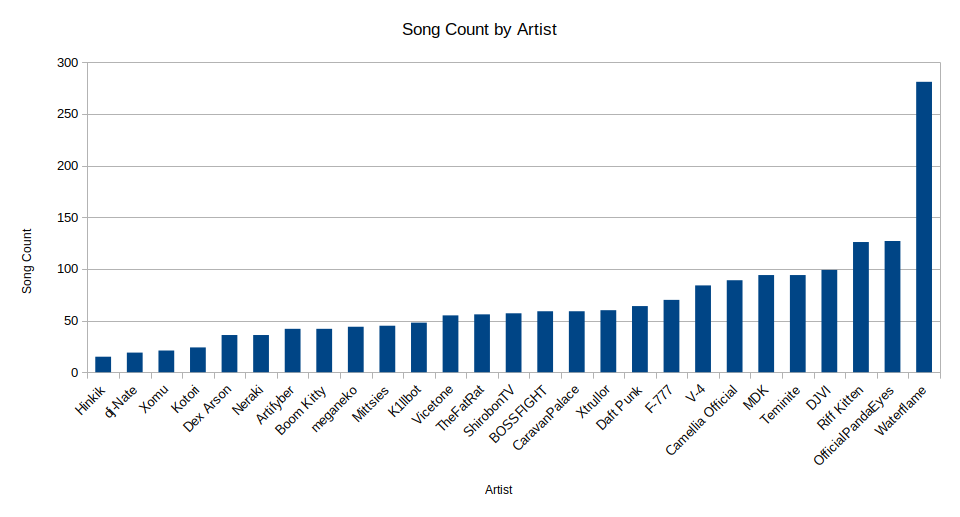
\includegraphics[width=0.95\textwidth]{resources/count_by_artist.png}}
\caption{Bar chart displaying number of songs uploaded by each artist.}
\label{figure_byArtistCount}
\end{figure*}

\begin{figure*}
\centering
\frame{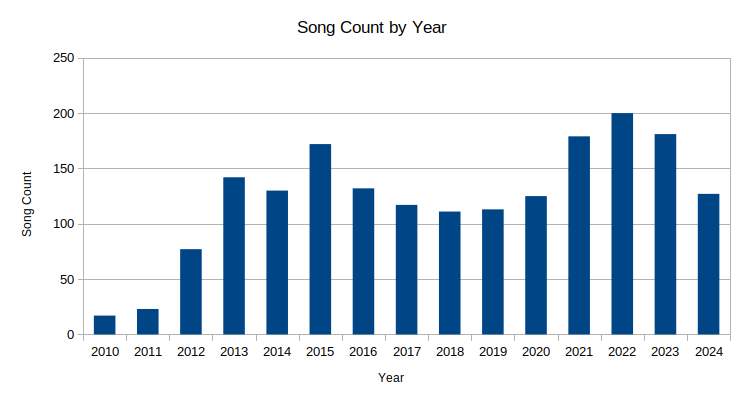
\includegraphics[width=0.95\textwidth]{resources/count_by_year.png}}
\caption{Bar chart displaying number of songs uploaded each year from 2010 to 2024.}
\label{figure_byYearCount}
\end{figure*}

% initial analysis techniques
Initial exploration of the dataset was performed using Weka 3.8.6. A new CSV file had to be created to 1) reduce the number of columns to 100 for performance reasons, prioritizing the most informative features, and 2) remove filenames as the presence of certain characters prevented Weka from fully reading the file. All using 10-fold cross-validation, \code{ZeroR} classification correctly classified the \textbf{artist} of 15.5\% of the instances; \code{OneR} correctly classified 17.0\% of instances; \code{RandomForest} correctly classified 50.9\% of instances; and \code{SimpleLogistic} correctly classified 59.2\% of the total instances. Refer to the confusion matrix in Table \ref{table_cm1}. 59.2\% accuracy using \code{SimpleLogistic} compared to the 15.5\% of randomly guessing using \code{ZeroR} is promising and strongly suggests the existence of meaningful patterns within the dataset to distinguish between artists' styles. Also all using 10-fold cross-validation, \code{ZeroR} classification correctly classified the \textbf{year} of 10.8\% of the instances; \code{OneR} correctly classified 11.9\% of instances; \code{RandomForest} correctly classified 24.5\% of instances; and \code{SimpleLogistic} correctly classified 20.4\% of the total instances. In this case, \code{RandomForest} outperformed \code{SimpleLogistic}, while both performed much better than random, this result is likely skewed by disproportionate contributions to the dataset by artists across the years. Refer to the confusion matrix in Table \ref{table_cm2}.

% todo determine how to center this
% Table generated using: https://github.com/TidiaTDA/ConfWeka2LaTex/blob/main/main.py
\begin{table}[htp]
\centering
\setlength{\tabcolsep}{0.05em}
\begin{tabular}{|| c | c c c c c c c c c c c c c c c c c c c c c c c c c c c ||}
\hline
Artifyber & \textbf{17} & 0 & 0 & 4 & 1 & 1 & 0 & 1 & 1 & 3 & 0 & 0 & 0 & 0 & 1 & 2 & 2 & 3 & 1 & 0 & 0 & 0 & 1 & 0 & 3 & 0 & 1 \\ 
BoomKitty & 0 & \textbf{24} & 1 & 1 & 0 & 1 & 0 & 0 & 0 & 1 & 0 & 0 & 0 & 1 & 1 & 0 & 2 & 1 & 0 & 3 & 5 & 0 & 0 & 0 & 1 & 0 & 0 \\ 
BOSSFIGHT & 1 & 2 & \textbf{19} & 3 & 0 & 1 & 1 & 1 & 3 & 0 & 1 & 0 & 1 & 6 & 2 & 1 & 1 & 3 & 0 & 3 & 1 & 0 & 0 & 1 & 3 & 0 & 5 \\ 
CamelliaOfficial & 3 & 1 & 1 & \textbf{74} & 0 & 0 & 1 & 0 & 0 & 0 & 0 & 0 & 0 & 1 & 1 & 0 & 1 & 1 & 0 & 2 & 2 & 0 & 0 & 0 & 0 & 1 & 0 \\ 
CaravanPalace & 1 & 0 & 0 & 1 & \textbf{38} & 3 & 0 & 0 & 0 & 0 & 0 & 0 & 1 & 0 & 0 & 1 & 0 & 1 & 4 & 0 & 1 & 3 & 0 & 3 & 1 & 0 & 1 \\ 
DaftPunk & 2 & 0 & 0 & 0 & 7 & \textbf{29} & 0 & 0 & 2 & 2 & 0 & 2 & 0 & 4 & 0 & 4 & 0 & 0 & 6 & 0 & 0 & 0 & 1 & 0 & 2 & 2 & 1 \\ 
DexArson & 0 & 0 & 0 & 0 & 0 & 0 & \textbf{15} & 2 & 1 & 2 & 0 & 2 & 1 & 3 & 0 & 0 & 0 & 6 & 0 & 0 & 3 & 0 & 0 & 0 & 0 & 0 & 1 \\ 
djNate & 0 & 0 & 1 & 0 & 0 & 1 & 3 & \textbf{7} & 0 & 0 & 0 & 0 & 0 & 1 & 0 & 0 & 0 & 2 & 0 & 0 & 0 & 1 & 0 & 0 & 2 & 0 & 1 \\ 
DJVI & 1 & 1 & 0 & 0 & 0 & 1 & 1 & 0 & \textbf{71} & 3 & 0 & 0 & 0 & 0 & 1 & 0 & 0 & 1 & 0 & 1 & 1 & 2 & 3 & 3 & 5 & 4 & 0 \\ 
F777 & 2 & 1 & 1 & 2 & 0 & 0 & 2 & 0 & 3 & \textbf{36} & 0 & 1 & 0 & 8 & 0 & 0 & 1 & 2 & 0 & 0 & 0 & 1 & 3 & 0 & 4 & 1 & 2 \\ 
Hinkik & 0 & 0 & 0 & 1 & 0 & 0 & 0 & 0 & 0 & 1 & \textbf{2} & 1 & 0 & 1 & 0 & 0 & 0 & 1 & 0 & 0 & 3 & 0 & 0 & 4 & 0 & 0 & 1 \\ 
K1llbot & 1 & 0 & 1 & 1 & 0 & 3 & 0 & 0 & 0 & 0 & 1 & \textbf{25} & 1 & 1 & 1 & 0 & 2 & 3 & 1 & 1 & 2 & 0 & 1 & 0 & 1 & 0 & 2 \\ 
Kotori & 0 & 0 & 3 & 0 & 0 & 0 & 0 & 0 & 0 & 0 & 0 & 0 & \textbf{14} & 0 & 0 & 0 & 1 & 5 & 0 & 0 & 0 & 0 & 0 & 0 & 0 & 0 & 1 \\ 
MDK & 0 & 0 & 2 & 2 & 1 & 0 & 1 & 1 & 4 & 4 & 1 & 0 & 1 & \textbf{42} & 3 & 1 & 3 & 4 & 0 & 2 & 6 & 1 & 2 & 0 & 8 & 0 & 5 \\ 
meganeko & 0 & 0 & 3 & 1 & 0 & 0 & 0 & 0 & 2 & 0 & 1 & 0 & 0 & 3 & \textbf{12} & 1 & 1 & 4 & 0 & 3 & 2 & 4 & 0 & 1 & 5 & 0 & 1 \\ 
Mittsies & 1 & 0 & 0 & 0 & 0 & 1 & 0 & 0 & 0 & 0 & 0 & 1 & 0 & 0 & 0 & \textbf{35} & 0 & 0 & 2 & 1 & 0 & 0 & 1 & 0 & 3 & 0 & 0 \\ 
Neraki & 0 & 2 & 0 & 3 & 0 & 0 & 0 & 0 & 0 & 3 & 0 & 0 & 2 & 2 & 0 & 0 & \textbf{14} & 0 & 0 & 0 & 5 & 0 & 0 & 0 & 4 & 0 & 1 \\ 
OfficialPandaEyes & 0 & 0 & 4 & 1 & 3 & 2 & 6 & 1 & 0 & 6 & 0 & 1 & 3 & 6 & 1 & 1 & 1 & \textbf{73} & 1 & 0 & 6 & 5 & 0 & 2 & 1 & 0 & 3 \\ 
RiffKitten & 0 & 0 & 0 & 0 & 6 & 9 & 0 & 0 & 0 & 0 & 0 & 0 & 0 & 0 & 0 & 0 & 0 & 2 & \textbf{83} & 2 & 2 & 2 & 2 & 4 & 14 & 0 & 0 \\ 
ShirobonTV & 3 & 0 & 1 & 2 & 3 & 1 & 0 & 1 & 1 & 0 & 0 & 0 & 1 & 4 & 3 & 1 & 0 & 3 & 0 & \textbf{23} & 0 & 3 & 0 & 0 & 7 & 0 & 0 \\ 
Teminite & 0 & 2 & 2 & 2 & 0 & 0 & 5 & 0 & 5 & 1 & 0 & 0 & 1 & 4 & 0 & 0 & 2 & 9 & 3 & 0 & \textbf{51} & 2 & 0 & 1 & 2 & 1 & 1 \\ 
TheFatRat & 0 & 0 & 0 & 0 & 4 & 1 & 0 & 1 & 2 & 0 & 0 & 0 & 0 & 4 & 2 & 0 & 0 & 5 & 6 & 2 & 0 & \textbf{19} & 0 & 6 & 2 & 2 & 0 \\ 
V4 & 0 & 3 & 0 & 0 & 0 & 0 & 0 & 0 & 1 & 1 & 0 & 1 & 0 & 0 & 0 & 1 & 0 & 0 & 0 & 0 & 0 & 1 & \textbf{68} & 0 & 7 & 0 & 1 \\ 
Vicetone & 0 & 0 & 0 & 0 & 2 & 0 & 0 & 0 & 2 & 0 & 1 & 1 & 0 & 0 & 1 & 0 & 0 & 1 & 3 & 1 & 0 & 4 & 0 & \textbf{36} & 0 & 2 & 1 \\ 
Waterflame & 1 & 3 & 2 & 4 & 1 & 4 & 0 & 1 & 4 & 1 & 0 & 0 & 0 & 1 & 1 & 4 & 2 & 0 & 14 & 2 & 2 & 1 & 6 & 0 & \textbf{231} & 0 & 1 \\ 
Xomu & 0 & 0 & 0 & 0 & 1 & 0 & 0 & 0 & 1 & 0 & 0 & 0 & 0 & 0 & 0 & 0 & 0 & 3 & 1 & 0 & 2 & 4 & 0 & 3 & 0 & \textbf{6} & 0 \\ 
Xtrullor & 0 & 0 & 0 & 1 & 0 & 2 & 1 & 0 & 0 & 0 & 0 & 1 & 1 & 3 & 3 & 0 & 4 & 3 & 0 & 0 & 3 & 0 & 1 & 2 & 2 & 1 & \textbf{32} \\ [1ex]
\hline
\end{tabular}
\caption{Confusion matrix for artists using 10-fold cross-validation SimpleLogistic classification.}
\label{table_cm1}
\end{table}

% Table generated using: https://github.com/TidiaTDA/ConfWeka2LaTex/blob/main/main.py
\begin{table}[htp]
\centering
\setlength{\tabcolsep}{0.3em}
\begin{tabular}{|| c | c c c c c c c c c c c c c c c ||}
\hline
2010\  & \textbf{0} & 0 & 2 & 2 & 3 & 4 & 0 & 0 & 0 & 0 & 1 & 3 & 1 & 0 & 1 \\ 
2011\  & 0 & \textbf{0} & 1 & 4 & 3 & 9 & 1 & 0 & 0 & 0 & 0 & 1 & 3 & 1 & 0 \\ 
2012\  & 0 & 1 & \textbf{9} & 10 & 2 & 15 & 5 & 1 & 1 & 2 & 5 & 7 & 13 & 6 & 0 \\ 
2013\  & 0 & 0 & 5 & \textbf{51} & 12 & 33 & 7 & 2 & 1 & 0 & 2 & 5 & 16 & 8 & 0 \\ 
2014\  & 0 & 0 & 3 & 24 & \textbf{22} & 30 & 2 & 7 & 1 & 6 & 6 & 8 & 14 & 6 & 1 \\ 
2015\  & 0 & 0 & 1 & 15 & 15 & \textbf{63} & 15 & 6 & 0 & 11 & 7 & 14 & 14 & 5 & 6 \\ 
2016\  & 0 & 0 & 2 & 10 & 4 & 31 & \textbf{23} & 7 & 6 & 6 & 4 & 15 & 16 & 5 & 3 \\ 
2017\  & 0 & 0 & 0 & 10 & 6 & 19 & 16 & \textbf{11} & 3 & 4 & 11 & 13 & 15 & 8 & 1 \\ 
2018\  & 0 & 0 & 0 & 8 & 8 & 16 & 9 & 2 & \textbf{13} & 8 & 5 & 12 & 17 & 11 & 2 \\ 
2019\  & 0 & 0 & 1 & 2 & 3 & 14 & 8 & 4 & 4 & \textbf{19} & 10 & 23 & 16 & 5 & 4 \\ 
2020\  & 0 & 0 & 2 & 4 & 3 & 11 & 7 & 2 & 1 & 11 & \textbf{34} & 22 & 14 & 12 & 2 \\ 
2021\  & 0 & 0 & 1 & 10 & 7 & 12 & 8 & 2 & 5 & 9 & 13 & \textbf{49} & 30 & 29 & 4 \\ 
2022\  & 0 & 0 & 0 & 10 & 5 & 15 & 10 & 5 & 5 & 4 & 11 & 24 & \textbf{86} & 22 & 3 \\ 
2023\  & 0 & 0 & 3 & 15 & 10 & 9 & 4 & 3 & 3 & 3 & 11 & 34 & 27 & \textbf{54} & 5 \\ 
2024\  & 0 & 0 & 0 & 4 & 4 & 14 & 5 & 0 & 2 & 6 & 6 & 16 & 25 & 27 & \textbf{18} \\ [1ex]
\hline
\end{tabular}
\caption{Confusion matrix for years spanning 2010-2024 using 10-fold cross-validation RandomForest classification.}
\label{table_cm2}
\end{table}


% follow-on analysis
Although Scikit has already been used to select for informative features used in the dataset, using Weka to perform further feature selection using \code{Correlation}, \code{InfoGain}, and \code{OneR} attribute evaluation only commonly include \code{lowlevel.erbbands.median.4} among the 10 most informative features.


\section{Results}
% summary/standout key findings
From this low-cost and high-manual-effort dataset, it was found that, assuming the analysis was not derailed by a poor selection of a data source, that the represented artists styles' are quantifiably distinct from one another. Less compelling, but still better than random, evidence suggests that the broader EDM genre has evolved in the years since 2010 (though certainly since the 1960s).

% Clusters
Using Weka to perform \code{SimpleKMeans} clustering up to 7 clusters unilaterally resulted in incorrect clustering in at least 80\% of instances across all the cluster counts. The 2-cluster clustered around Riff Kitten and Waterflame which marks a distinction between electro-swing and chiptune/video-gamey music. N-clusters 3 through 5 additionally clustered around DJVI, MDK, and Panda Eyes, respectively, introducing more "typical" loud \& aggressive EDM styles. It was unexpected that it would take until 7 clusters to separate out Daft Punk as its own cluster given that are presumed to be the most mainstream artist within the dataset and their style is much more laid-back compared to the other artists.

% bossfight
A specific observation that inspired this choice of paper was that Bossfight's older music is drastically different than what they produce today (far less happy-go-lucky/energetic and much more loud/dramatic) - and this may not be a novel observation - but classification using Weka validates this line of thinking.  As Bossfight has only 59 entries in the dataset (3.9 per year) and there is a rather telling gap between 2012 and 2015, their entries were manually clustered to a 2011-2012 class, a 2015-2019 class, and a 2020-2024 class containing their newest tracks. \code{ZeroR} classification correctly classified 40.7\% of instances while \code{SimpleLogistic} classified a far greater 86.4\% to the correct cluster.

% time crunch - I otherwise would analyze more specific cases here...

\section{Conclusion}
% takeaways of the analysis
The two primary findings of this paper are that (Indie) EDM artists' styles are not merely qualitatively distinct from one another, and that the artist Bossfight has indeed redefined their musical signature. Features selected for within the reduced dataset may (or may not) point toward a greater understanding of EDM as a genre for those knowledgeable of the musical/audio meaning of the features extracted by Essentia.

% fix up yt method; use other platform
% use legit db to source music
% use existing db of musicological data
% follow-on broader set of artists; select for "popular"
% future work
The Achilles' heel of this analysis is whether or not sourcing MP3 files from Youtube, or by using YT-DLP specifically, introduced unintended patterns such as an audio watermark that oversimplified the classification process; it is uncertain how introducing data from a different source such as Spotify would affect this. A possible solution for this would be to pay for access to a professionally-maintained database, which would also potentially be better suited to random sampling rather than arbitrary identification \& selection of artists \& songs. Essentia's website links to applications of their tooling such as AcousticBrainz, which crowdsources acoustic data; making use of such already-available data might also be a major improvement upon the methodology established in this paper. Expansion upon the topic of EDM in particular could incorporate a broader variety of artists, though it is doubtful that continuing to use Youtube as a source for MP3 files would be prudent.


\section*{Acknowledgments}
Dr. Lior Shamir for a job well done teaching the concepts of Data Science Foundations during the Fall 2024 semester at Kansas State University and providing references on Essentia and LaTeX use.


\label{Bibliography}
\bibliography{main}
\bibliographystyle{apalike}



\end{document}



